% !TEX root = ../notes_unsupervisedlearning.tex
% Chapter 7: Uncertainty Estimation
%%%%%%%%%%%%%%%%%%%%%%%%%%%%%%%%%%%%%%%%%%%%%%%%%%%%%%%%%%%%%%%%%%%%%%

\chapter{Uncertainty Estimation}\index{Uncertainty Estimation}\index{epistemic uncertainty}\index{aleatoric uncertainty}\index{Anomaly Detection}\index{OOD Detection}
\newthought{I know that I know nothing.}

% ==============================================================================================
% BLOCK 1: INTRODUCTION
% ==============================================================================================

\section{The Why}\index{uncertainty estimation}



\newthought{In the previous chapter} we learned to compress high-dimensional data into structured latent spaces and embeddings\index{embedding}\index{feature space}
and even to draw new samples from those spaces. Closing we even explored and stepped through the latent feature space itself.
Neither capability told us how much we should trust those embeddings or outputs for any particular input.
A reconstruction\index{reconstruction error} looks the same whether the embedding lay in the heart of the training distribution or far from any encoded
neighbour in feature space; the model has no built-in way to communicate its own uncertainty.



\marginnote{\newthought{Neural networks} are trained to predict, and they do so with impressive accuracy on familiar data, 
which makes them particularly misleading on unfamiliar data.}

\newthought{The Confidence Value and Prediction Probabilities are ambiguous.}
Neural networks calibrate poorly on out-of-distribution inputs by design: the softmax\index{softmax confidence} normalises to sum to one.
Confidence collapses to a measure of similarity within the known domain itself and fails out-of-domain distributions.
As a consequence we need to establish ways to determine the actual confidence we have in a model.

\marginnote{\newthought{Adversarial inputs}\index{adversarial inputs} lift the problem to a sharper edge, where the model
is high-confidence wrong on imperceptible perturbations.}



% Move this into the theory main block on a later run next year.
\newthought{Calibration}\index{calibration}\cite{Guo2017Calibration}. In a supervised setting the accuracy of the model is known, and using that information
the confidence can be calibrated by the actual accuracy in a specific confidence bin.

\newthought{Confidence Head.}\index{confidence head}
A complementary route is to train a small head whose only job is to predict
whether the main model is actually confident to be right on the current input,
turning the model's own likelihood of being correct into a prediction target.

\newthought{Confidence by Reconstruction.}\index{reconstruction error}\index{VAE}
In the spirit of the Variational Autoencoder Architecture, the confidence in an embedding
gets varified when its reconstruction gets compared with its decoding. Even when out of domain samples fall within the
latent feature space of our training data, the reconstruction collapses onto the training domain, highlighting out of domain samples.


\marginnote{\newthought{The heavy tail of aleatoric uncertainty.}\cite{Koopman2018HeavyTail} Real-world data is heavy-tailed: A small number 
of common situations cover most of the volume, but a long tail of rare configurations refuses to vanish no matter how 
much data is collected. Autonomous vehicles thus have no means to have learned those rare events, 
so at least they need to realize that they move out of domain.}

\newthought{Epistemic Uncertainty.}\index{epistemic uncertainty}
While uncertainty within the data, which is called aleatoric, is a concern the models own uncertainty is
the focus when brought to application. Introducting noise\index{noise} into our learned parameters during inference,
the variance\index{variance} in prediction result is measured and used as an indicator for uncertainty. This approach is the basis for 
Monte Carlo Dropout\index{Monte Carlo Dropout}.



% A complementary thread is explainability\index{explainable AI}\cite{Ribeiro2016LIME}: when a flagged decision is shown to a reviewer, surfacing the features or training neighbours that drove the prediction tells them where to look, so calibration tells the reviewer when to look and explanation tells them what to look at.

\newthought{Application and Acting under uncertainty}. 
Uncertainty estimations turn confidence into a signal that informs our downstream modules.



\marginnote{\newthought{ODD and drift.}\index{operational design domain}\index{distribution shift} The operational design domain 
names the conditions under which a system was designed to work, 
namely the slice of the world the training data covered. 
ODD detection asks at runtime whether the current input falls inside that slice. 
Data drift is the slow change in input statistics over time; 
model drift is the resulting decoupling of stated confidence from empirical accuracy.}

\marginnote{\newthought{Anomaly Detection and On-Domain Learning.} Making a virtue of necessity. 
We can use uncertainty estimates for anomaly detection on one-class 
embeddings\index{one-class learning}: Deliberately fit only normal data, then flag any input the model finds unusual
without ever showing it a labelled anomaly.} 





\newthought{In order to move from overconfident predictors to uncertainty estimations} we have good reason to find ways to,
\begin{itemize}
    \item separate aleatoric from epistemic uncertainty, so that each source informs the predictive confidence of our model.
    \item measure or predict model uncertainty in out of domain distributions.
    \item act on uncertainty estimates in practice, routing unreliable predictions to human reviewers, falling back to fail-safe defaults, and detecting inputs the model was never trained to handle.
\end{itemize}




\newpage
\iffalse

\subsection{Hands On Experience}

\newthought{Step into the role of the classifier.}
Imagine you have just finished a clustering pass over a training set and the result you walk away with is binding: there are exactly two classes in the world, the cluster on the left and the cluster on the right.
We will hand you grey candidates one at a time and your job is to commit each one to either left or right.
You are not allowed to abstain, you are not allowed to invent a third option, and you have to give an answer for every point we show you.
Read Figure~\ref{fig:uncertainty_intro} as the world the rules describe: ten training points define what a class looks like, and four grey candidates wait for your verdict.

\begin{figure}
\centering
\begin{tikzpicture}
    \begin{axis}[
        xlabel={$x^{(1)}$}, ylabel={$x^{(2)}$},
        xmin=-1, xmax=8, ymin=-1, ymax=6,
        width=0.5\textwidth, height=0.5\textwidth,
        axis line style={draw=none},
        tick style={black, thick},
        xtick={0,2,4,6}, ytick={0,2,4},
        xticklabel style={font=\small},
        yticklabel style={font=\small},
        tick align=outside, tick pos=left,
    ]
    \addplot[only marks, mark=*, mark size=2pt, black] coordinates {
        (2,2) (2.5,2.3) (2.2,2.8) (3,2.5) (2.8,2) (2.3,2.5)
        (2.7,2.2) (2.4,2.7) (2.1,2.4) (2.6,2.6)
    };
    \addplot[only marks, mark=*, mark size=2pt, black!30] coordinates {
        (3.5,3.2) (6,1) (1,5) (7,4)
    };
    \node[font=\small] at (axis cs:3.5,3.7) {?};
    \node[font=\small] at (axis cs:6,0.5) {?};
    \node[font=\small] at (axis cs:1,5.5) {?};
    \node[font=\small] at (axis cs:7,4.5) {?};
    \end{axis}
\end{tikzpicture}
\caption{Ten training points clustered around $(2.5, 2.5)$ in black define the only two classes the rules permit; four grey candidates sit outside that cluster at varying distances and directions. The candidate at $(3.5, 3.2)$ is an easy commit, the candidates at $(6, 1)$ and $(1, 5)$ are borderline in opposite directions, and the candidate at $(7, 4)$ sits far enough out that the rules feel wrong.}
\label{fig:uncertainty_intro}
\end{figure}

\newthought{The first candidate is easy.}
The grey point at $(3.5, 3.2)$ sits a hair outside the dense cloud, in the direction the cluster is already trending.
You commit it to the same class without much hesitation, and your internal confidence is high.
This is the regime classifiers are built for: the input looks like the training data, the answer is the obvious one, and there is no friction between the rules and your intuition.

\newthought{The borderline pair is uncomfortable.}
The candidate at $(6, 1)$ sits well to the right, away from anything you have seen, and the candidate at $(1, 5)$ sits well above the cluster in a different direction entirely.
The rules still demand a single class, so you commit, but the commitment now feels arbitrary: nothing in the data tells you these two grey points belong together, only the impoverished label set does.
Notice that you have just produced two predictions whose internal confidence has dropped sharply, and yet a softmax over two classes will normalise to one regardless and give you no place to record that drop.

\marginnote{\newthought{Open questions for the role-play.}
\begin{itemize}
    \item Which candidate did you commit with the most discomfort, and what would you have written next to that prediction if you had been allowed?
    \item If the points at $(6, 1)$ and $(1, 5)$ both became their own new classes tomorrow, what would change in your earlier commitments?
    \item How would you, as a system designer, prevent a downstream actuator from acting on the $(7, 4)$ commitment with the same trust as the $(3.5, 3.2)$ one?
\end{itemize}}

\newthought{The far outlier breaks the rules.}
The candidate at $(7, 4)$ sits far enough from either training neighbourhood that the obvious answer is none of the above, and at this point we tell you what you already suspected: this point is a new class emerging in the wild, a regime your training pass never covered.
Your earlier commitment was forced and wrong, but the wrongness was never visible in the prediction itself, only in the gap between the input and everything you had ever seen.
This is the silent-failure mode from the section above made tactile: the loop closed around your answer and there was no flag to open it back up.

\newthought{Now for the second twist.}
We come back and reveal that the ten training points were never one class at all: the lower band around $y \approx 2$ and the upper band around $y \approx 2.7$ have been two distinct subclasses since the beginning, and the clustering pass simply failed to resolve them.
Your earlier commitment to $(3.5, 3.2)$ now needs to split into two different answers depending on which subclass it should belong to, except you no longer have access to that earlier prediction in a form you can re-route.
The same trap shows up in deployment as slow drift: the world your model was trained on was already richer than your label set admitted, and the bill comes due once the richness becomes operationally relevant.

\newthought{Step out of the role and design the missing pieces.}
What the exercise made absent is exactly what an uncertainty-aware system has to provide.
First, an I-am-not-sure flag the model can raise when its commitment is forced rather than confident, so the borderline pair never travels downstream with the same trust as the easy commit.
Second, a routing rule that sends flagged inputs to a human reviewer who can override, defer, or label them as something new, turning the human-in-the-loop layer of the section above into a concrete pipeline stage.
Third, a novelty detector that watches for inputs unlike anything in the training distribution, so the $(7, 4)$ kind of point is recognised as new before it is forced into an existing class.
Fourth, a drift monitor that tracks the population of inputs and predictions over time, so that a slow subclass split is caught while it is still a small distortion of the calibration plot rather than a system-wide breakdown.

\newthought{Uncertainty estimation surfaces the gap.}
The same prediction now comes with a measure of doubt that downstream code can act on.
Instead of one number we get a structured signal: a mean prediction and a variance, a posterior over weights, or a per-input score that says how unusual this input looks compared to what the model was trained on.
That signal is what powers the four capabilities above, and the rest of this chapter is the toolkit for producing it.

\begin{marginfigure}
\centering
\begin{tikzpicture}
    \begin{axis}[
        xlabel={class probability},
        ylabel={density},
        xmin=0, xmax=1,
        ymin=0, ymax=10,
        width=\marginparwidth, height=0.7\marginparwidth,
        axis line style={draw=none},
        tick style={black, thin},
        xtick={0,0.5,1},
        ytick=\empty,
        xticklabel style={font=\tiny},
        xlabel style={font=\tiny},
        ylabel style={font=\tiny},
        tick align=outside, tick pos=left,
        samples=80,
        domain=0:1,
    ]
    \addplot[black, thick] {12*exp(-((x-0.85)^2)/0.005)};
    \addplot[black!55, thick, densely dashed] {3.5*exp(-((x-0.5)^2)/0.06)};
    \node[font=\tiny, anchor=south] at (axis cs:0.83,7.2) {peaked};
    \node[font=\tiny, black!55, anchor=south] at (axis cs:0.5,3.8) {flat};
    \end{axis}
\end{tikzpicture}
\caption{Two prediction profiles for the same kind of input. Solid: peaked, no uncertainty signal. Dashed: flat, high epistemic uncertainty. Both predict the same top class, but only the second tells you the model is unsure.}
\label{fig:profile_overlay}
\end{marginfigure}

\vspace{2.5em}

\newthought{The Learning Objectives} of this lecture:
\begin{itemize}
    \item Distinguish aleatoric from epistemic uncertainty and explain why only the latter is reducible with more data.
    \item Apply MC Dropout and Deep Ensembles to quantify prediction uncertainty, and turn that uncertainty into anomaly and out-of-distribution scores.
    \item Design graceful degradation strategies that route uncertain predictions to human reviewers and abstain when the model has no business answering.
\end{itemize}












% ==============================================================================================
% BLOCK 2: MAIN THEORY
% ==============================================================================================

\newpage

\subsection{Sources of Uncertainty}\index{aleatoric uncertainty}\index{epistemic uncertainty}

\marginnote{\newthought{Not all uncertainty is the same,} and the distinction determines what we can do about it. One kind we have to live with; the other we can chase down.}

\newthought{Two kinds of uncertainty} arise in any model trained on finite data.
The distinction is not pedantic; it determines whether collecting more data will help, whether retraining is worth the effort, and whether the right response is to flag the prediction or to commission new annotations.

\newthought{Aleatoric uncertainty}\index{aleatoric uncertainty} is inherent noise\index{noise} in the data and cannot be reduced by collecting more of it.
A sensor with finite precision will always introduce measurement noise; the same input handed to the system twice will produce two slightly different feature vectors, and no model on either of them can eliminate the spread.
Overlapping class boundaries are the same story: when two classes genuinely share regions of the input space, the optimal classifier is a probability, not a label, and the irreducible width of that probability is the aleatoric uncertainty.

\newthought{The aleatoric ceiling} is what a perfect model would still face after seeing infinite data.
Calling a coin flip is not hard because the coin is mysterious; it is hard because the outcome is genuinely random conditional on the input.
No amount of training data, no model class, no clever architecture lifts that ceiling.
The only thing the model can do is report the irreducible width honestly.

\newthought{Epistemic uncertainty}\index{epistemic uncertainty} reflects the model's ignorance and shrinks as more data arrives.
A model trained on summer temperatures has high epistemic uncertainty about winter; show it winter data and the uncertainty decreases.
A model trained on natural images has high epistemic uncertainty about satellite imagery; pre-train on satellite imagery, and that gap closes.
Epistemic uncertainty is the actionable kind: it tells us where the model needs more evidence and where collecting more data will pay off.

\newthought{The same input can carry both kinds at once.}
A medical image taken with a noisy sensor at the boundary between two tissue types carries aleatoric noise from the sensor and the boundary, and epistemic uncertainty from the lab not yet having labelled enough images of that boundary.
Quantifying each separately lets the deployed system route correctly: aleatoric uncertainty triggers a request for a second scan, epistemic uncertainty triggers a request for an expert label.

\begin{figure}
\centering
\begin{tikzpicture}
    \begin{axis}[
        xmin=-1, xmax=11, ymin=-1, ymax=11,
        width=0.5\textwidth, height=0.5\textwidth,
        axis line style={draw=none},
        tick style={black, thin},
        xtick=\empty, ytick=\empty,
        tick align=outside, tick pos=left,
    ]
    \addplot[only marks, mark=*, mark size=1.5pt, black] coordinates {
        (3,3) (3.4,3.6) (2.8,3.2) (3.2,2.7) (3.6,3.0)
        (4.0,3.4) (4.4,3.7) (4.8,4.1) (5.2,4.5) (5.6,4.8)
        (4.6,4.2) (5.0,3.9) (3.8,3.3) (4.2,3.8) (5.4,4.6)
    };
    \addplot[only marks, mark=*, mark size=1.5pt, black!55] coordinates {
        (5.0,5.4) (5.4,5.7) (5.8,6.0) (6.2,6.4) (6.6,6.7)
        (5.6,6.1) (6.0,5.8) (6.4,6.2) (6.8,6.5) (7.2,6.9)
        (5.2,5.8) (5.7,6.3) (6.1,5.6) (6.5,6.0) (7.0,6.7)
    };
    \draw[densely dashed, black!60] (axis cs:2,7) -- (axis cs:8,1);
    \node[font=\small, anchor=south west] at (axis cs:5.0,5.3) {overlap};
    \end{axis}
\end{tikzpicture}
\caption{Aleatoric uncertainty: two classes overlap in feature space. The dashed line is the optimal decision boundary, but inside the overlap region the optimal classifier returns a probability, not a label. The irreducible width of that probability is the aleatoric uncertainty.}
\label{fig:aleatoric_overlap}
\end{figure}

\begin{figure}
\centering
\begin{tikzpicture}
    \begin{axis}[
        xmin=-1, xmax=11, ymin=-1, ymax=11,
        width=0.5\textwidth, height=0.5\textwidth,
        axis line style={draw=none},
        tick style={black, thin},
        xtick=\empty, ytick=\empty,
        tick align=outside, tick pos=left,
    ]
    \addplot[only marks, mark=*, mark size=1.5pt, black] coordinates {
        (2,2) (2.3,2.4) (2.5,2.0) (2.7,2.5) (2.4,2.8)
        (3.0,2.2) (3.2,2.6) (2.8,3.0) (2.6,2.3) (3.1,2.4)
    };
    \addplot[only marks, mark=*, mark size=1.5pt, black!30] coordinates {
        (8,8)
    };
    \node[font=\small, anchor=west] at (axis cs:8.3,8) {?};
    \addplot[black!40, dashed, thin, domain=0:360, samples=40]
        ({2.65 + 1.0*cos(x)}, {2.45 + 1.0*sin(x)});
    \end{axis}
\end{tikzpicture}
\caption{Epistemic uncertainty: a familiar cluster of training points plus an isolated grey candidate sitting far from anything the model has seen. The dashed circle is the model's effective neighbourhood of confident predictions; outside it, the model's doubt is reducible by collecting more data.}
\label{fig:epistemic_sparse}
\end{figure}

\marginnote{\newthought{Calibration vs confidence.}\index{calibration} Calibration asks whether the model's stated probabilities match the empirical frequencies; a $90\%$ confidence prediction should be right $90\%$ of the time. Confidence is the raw number the model returns. A well-calibrated model can still be uncertain; a confident model can still be miscalibrated.}

\newthought{The practical consequence} is that these two sources call for different responses.
High aleatoric uncertainty means the problem is inherently hard at that point; the best strategy is to acknowledge the ambiguity and communicate it downstream so a human, or a redundant sensor, can decide.
High epistemic uncertainty means the model has not seen enough relevant data; the best strategy is to collect more data, or to flag the prediction as unreliable until more data arrives.

\newthought{Notice that aleatoric uncertainty is irreducible.}
Once we accept that, all our optimisation effort focuses on epistemic uncertainty: estimating it, shrinking it, and routing on it.
The next subsection asks how to measure epistemic uncertainty when all we have is a trained model and a single test input.


\subsection{Quantifying Epistemic Uncertainty}\index{Monte Carlo Dropout}\index{deep ensembles}

\marginnote{\newthought{Knowing what you do not know} is essential for safe deployment. Two methods do most of the work in practice.}

\newthought{If aleatoric uncertainty is hopeless,} we focus our estimation effort on epistemic uncertainty.
Two methods do most of the work in practice: Monte Carlo Dropout, which uses a single trained network with dropout enabled at test time, and Deep Ensembles, which trains several independent networks and aggregates their predictions.
Both produce a distribution over predictions for a given input, from which a mean and a variance can be read off.

\newthought{Monte Carlo Dropout}\index{Monte Carlo Dropout}\index{dropout}\cite{GalGhahramani2016} estimates epistemic uncertainty by running $T$ forward passes through the trained network with dropout enabled at test time.
Each dropout mask zeroes out a different subset of activations, producing a different sub-network.
The collection of $T$ predictions approximates a posterior over network weights; the spread across passes is an estimate of how much the prediction would change under plausible alternative weights.

\vspace{1.5em}

\begin{algorithm}[H]
\caption{Monte Carlo Dropout for epistemic uncertainty}
\begin{algorithmic}[1]
\Require Input $x$, network $f_\theta$ with dropout layers, number of passes $T$
\Ensure Mean prediction $\bar{y}$ and predictive variance $\mathrm{Var}(\hat{y})$
\For{$t = 1$ to $T$}
    \State $\hat{y}_t \gets f_\theta(x)$ \Comment{forward pass with dropout enabled}
\EndFor
\State $\bar{y} \gets \tfrac{1}{T} \sum_{t=1}^{T} \hat{y}_t$
\State $\mathrm{Var}(\hat{y}) \gets \tfrac{1}{T} \sum_{t=1}^{T} (\hat{y}_t - \bar{y})^2$
\end{algorithmic}
\end{algorithm}

\newthought{Notice that the only dial we control is $T$.}
More passes give a smoother estimate of mean and variance, at linear cost in inference time.
Inputs well-represented in the training data produce consistent predictions across masks; inputs far from the training distribution produce scattered, disagreeing predictions, and the variance grows.

\begin{figure}
\centering
\begin{tikzpicture}
    \begin{axis}[
        xlabel={pass $t$}, ylabel={$p(\text{class 1})$},
        xmin=0.5, xmax=5.5, ymin=0, ymax=1,
        width=0.5\textwidth, height=0.4\textwidth,
        axis line style={draw=none},
        tick style={black, thin},
        xtick={1,2,3,4,5}, ytick={0,0.5,1},
        xticklabel style={font=\small},
        yticklabel style={font=\small},
        xlabel style={font=\small},
        ylabel style={font=\small},
        tick align=outside, tick pos=left,
    ]
    \addplot[only marks, mark=*, mark size=2pt, black] coordinates {(1,0.86) (2,0.84) (3,0.88) (4,0.85) (5,0.87)};
    \draw[densely dashed, black!60] (axis cs:0.5,0.86) -- (axis cs:5.5,0.86);
    \node[font=\small, anchor=south west] at (axis cs:3.6,0.92) {$\bar{p}{\approx}0.86$};
    \end{axis}
\end{tikzpicture}
\caption{MC Dropout across $T{=}5$ forward passes on an in-distribution input. Predictions cluster tightly around $0.86$ with variance below $0.001$; the model is confident.}
\label{fig:mcd_in_distribution}
\end{figure}

\begin{figure}
\centering
\begin{tikzpicture}
    \begin{axis}[
        xlabel={pass $t$}, ylabel={$p(\text{class 1})$},
        xmin=0.5, xmax=5.5, ymin=0, ymax=1,
        width=0.5\textwidth, height=0.4\textwidth,
        axis line style={draw=none},
        tick style={black, thin},
        xtick={1,2,3,4,5}, ytick={0,0.5,1},
        xticklabel style={font=\small},
        yticklabel style={font=\small},
        xlabel style={font=\small},
        ylabel style={font=\small},
        tick align=outside, tick pos=left,
    ]
    \addplot[only marks, mark=*, mark size=2pt, black!55] coordinates {(1,0.9) (2,0.4) (3,0.7) (4,0.5) (5,0.8)};
    \draw[densely dashed, black!60] (axis cs:0.5,0.66) -- (axis cs:5.5,0.66);
    \node[font=\small, anchor=south west] at (axis cs:3.6,0.72) {$\bar{p}{\approx}0.66$};
    \end{axis}
\end{tikzpicture}
\caption{MC Dropout across $T{=}5$ forward passes on an out-of-distribution input. Predictions scatter from $0.4$ to $0.9$ with variance above $0.03$; the mean is similar to the in-distribution case but the spread is the signal that flags this input as unfamiliar. Compare with Figure~\ref{fig:mcd_in_distribution}.}
\label{fig:mcd_out_distribution}
\end{figure}

\newthought{Each dropout mask produces a different sub-network} drawn from a Bernoulli distribution over which activations are kept.
Gal and Ghahramani showed that this matches a variational approximation\index{variational inference} to a Bayesian neural network\index{Bayesian neural network} with a specific prior over weights, so MC Dropout can be read as a cheap, after-the-fact approximation of a posterior we never explicitly trained.
The mean prediction is the posterior predictive mean; the variance is the posterior predictive variance.

\newthought{Deep ensembles}\index{deep ensembles}\cite{Lakshminarayanan2017} take the idea further by training $M$ independent models and aggregating their predictions:

\begin{align*}
    p(y \mid x) &= \tfrac{1}{M} \sum_{m=1}^{M} p_m(y \mid x)
\end{align*}

Disagreement among ensemble members signals epistemic uncertainty.
Unlike MC Dropout, each ensemble member is initialised and trained independently, so the diversity of predictions is driven by genuine differences in the learned representations rather than by random masking of a single trained model.
The price is the cost of $M$ training runs; the benefit is more reliable uncertainty estimates, especially on inputs far from the training distribution.

\begin{figure}
\centering
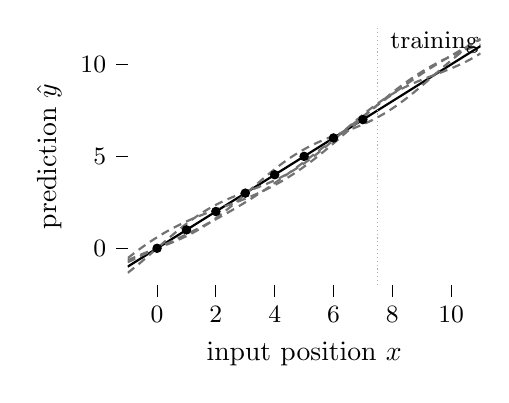
\begin{tikzpicture}
    \begin{axis}[
        xlabel={input position $x$}, ylabel={prediction $\hat{y}$},
        xmin=-1, xmax=11, ymin=-2, ymax=12,
        width=0.5\textwidth, height=0.4\textwidth,
        axis line style={draw=none},
        tick style={black, thin},
        xtick={0,2,4,6,8,10},
        ytick={0,5,10},
        xticklabel style={font=\small},
        yticklabel style={font=\small},
        tick align=outside, tick pos=left,
        samples=80,
        domain=-1:11,
    ]
    \addplot[black, thick] {x};
    \addplot[black!55, thick, densely dashed] {x + 0.4*sin(deg(x))};
    \addplot[black!55, thick, densely dashed] {x - 0.4*sin(deg(x))};
    \addplot[black!55, thick, densely dashed] {x + 0.6*cos(deg(0.7*x))};
    \addplot[black!55, thick, densely dashed] {x - 0.5*sin(deg(0.5*x))};
    \draw[black!30, densely dotted] (axis cs:7.5,-2) -- (axis cs:7.5,12);
    \node[font=\small, anchor=west] at (axis cs:7.6,11.2) {training ends};
    \addplot[only marks, mark=*, mark size=1.5pt, black] coordinates {
        (0,0)(1,1)(2,2)(3,3)(4,4)(5,5)(6,6)(7,7)
    };
    \end{axis}
\end{tikzpicture}
\caption{Five ensemble members on a one-dimensional regression. Inside the training range (left of the dotted line), the members agree closely. Outside it, they fan out, and the disagreement among ensemble predictions is the epistemic uncertainty estimate.}
\label{fig:ensemble_disagreement}
\end{figure}

\newthought{The choice between MC Dropout and Deep Ensembles} is a budget-versus-quality trade.
MC Dropout costs nothing to train (the network is already trained with dropout for regularisation) and $T$ forward passes at inference; the variance estimate is biased toward what dropout-induced perturbation can capture.
Deep Ensembles cost $M$ full training runs and $M$ forward passes at inference; the variance estimate captures genuine differences in learned representations and tracks epistemic uncertainty more faithfully on truly novel inputs.

\marginnote{\newthought{A practical protocol.} Pick MC Dropout when only one training run is affordable, when inference latency is loose, and when the network already uses dropout. Pick Deep Ensembles when accuracy and calibration are critical, training compute is available, and you can serve $M$ inference passes per query. For very large models where neither is affordable, use a small ensemble of $M{=}3$ to $M{=}5$ networks, each with MC Dropout at inference, to combine the two diversities cheaply.}

\marginnote{\newthought{The hard part is calibration.}\index{calibration} Even a well-quantified variance can be miscalibrated if the model overestimates its certainty. Temperature scaling\index{temperature scaling}, Platt scaling\index{Platt scaling}, and isotonic regression\index{isotonic regression} are post-hoc corrections that align stated probabilities with empirical frequencies. None of them shrink epistemic uncertainty; they make the estimate honest.}

\newthought{With epistemic uncertainty quantified,} we have a number per input that says how much the model would disagree with itself under reasonable variation.
The next question is what to do with that number: how does a variance translate into a decision?
That is the catalogue of scoring methods.


\subsection{Scoring Methods: From Uncertainty to Decisions}\index{Anomaly Detection}\index{OOD detection}

\marginnote{\newthought{Quantified uncertainty} becomes useful only when it drives a decision. Three families of scoring methods turn raw variance into actionable scores; a fourth family handles the special case where the input may not even be in-distribution.}

\newthought{Quantified uncertainty} becomes useful only when it drives a decision.
Three families of scoring methods translate the upstream uncertainty story into actionable scores: statistical scores, proximity-based scores, and reconstruction-based scores.
A fourth family, out-of-distribution detection, handles the special case where the input may not even belong to the training distribution at all.
All four families share the same logical structure: a function $s(x)$ that maps an input to a number, paired with a threshold above which the input is flagged.

\newthought{Anomaly detection}\index{Anomaly Detection}\cite{Chandola2009} asks whether individual observations deviate from a learned notion of normal.
The methods in this catalogue can be read as different ways of measuring how uncertain the model is about an input: through distributional assumptions, through proximity in feature space, or through reconstruction fidelity.
The choice between them depends on the type of anomaly we expect.

\vspace{1.5em}
\newthought{Types of anomalies.}\index{point anomaly}\index{contextual anomaly}\index{collective anomaly}
A taxonomy clarifies which detector to reach for.

\newthought{Point anomalies} are individual instances anomalous with respect to the rest of the data.
A single fraudulent transaction amid millions of legitimate ones is a point anomaly: nothing else in the dataset looks like it.

\newthought{Contextual anomalies} are instances anomalous only within a specific context.
A temperature of $30^{\circ}$C is normal in summer but anomalous in winter; the value itself is unremarkable, but the context makes it suspicious.
Detecting contextual anomalies requires features that encode the context, not just the raw observation.

\newthought{Collective anomalies} are collections of instances individually normal but together forming an anomalous pattern.
A sequence of login attempts from a hundred different countries within one hour is the canonical example; each login is normal, but the pattern is not.
Collective anomalies require the detector to look at sequences or groups, not single points.

\begin{figure}
\centering
\begin{tikzpicture}
    \begin{axis}[
        xmin=0, xmax=10, ymin=0, ymax=10,
        width=0.5\textwidth, height=0.4\textwidth,
        axis line style={draw=none},
        tick style={black, thin},
        xtick=\empty, ytick=\empty,
        tick align=outside, tick pos=left,
    ]
    \addplot[only marks, mark=*, mark size=2pt, black] coordinates {
        (3,3) (3.5,3.2) (3.2,3.5) (3.8,3.3) (3.3,3.7)
    };
    \addplot[only marks, mark=*, mark size=2pt, black!30] coordinates {(8,8)};
    \end{axis}
\end{tikzpicture}
\caption{Point anomaly. A single grey instance sits isolated from the cluster of normal points. The anomaly is detectable from the instance alone, without any context.}
\label{fig:anomaly_point}
\end{figure}

\begin{figure}
\centering
\begin{tikzpicture}
    \begin{axis}[
        xmin=0, xmax=10, ymin=0, ymax=10,
        width=0.5\textwidth, height=0.4\textwidth,
        axis line style={draw=none},
        tick style={black, thin},
        xtick=\empty, ytick=\empty,
        tick align=outside, tick pos=left,
    ]
    \addplot[black, thin] coordinates {(0,5) (3,5) (4,3) (6,3) (7,5) (10,5)};
    \addplot[only marks, mark=*, mark size=2pt, black!30] coordinates {(5,5)};
    \node[font=\small] at (axis cs:5,6.5) {context: dip};
    \end{axis}
\end{tikzpicture}
\caption{Contextual anomaly. The grey instance has a value that would be normal in many regions of the input, but the surrounding context, a dip in the signal, makes it suspicious.}
\label{fig:anomaly_contextual}
\end{figure}

\begin{figure}
\centering
\begin{tikzpicture}
    \begin{axis}[
        xmin=0, xmax=10, ymin=0, ymax=10,
        width=0.5\textwidth, height=0.4\textwidth,
        axis line style={draw=none},
        tick style={black, thin},
        xtick=\empty, ytick=\empty,
        tick align=outside, tick pos=left,
    ]
    \addplot[black, thin, domain=0:10, samples=50] {5 + 0.5*sin(deg(x*2))};
    \addplot[black!30, thick] coordinates {(4,5) (4.5,5.5) (5,4.5) (5.5,5.5) (6,4.5)};
    \end{axis}
\end{tikzpicture}
\caption{Collective anomaly. Each individual point in the highlighted segment is normal in isolation, but the oscillation pattern they form together is not part of the underlying signal.}
\label{fig:anomaly_collective}
\end{figure}

\vspace{2.5em}
\newthought{Statistical scoring.}\index{Z-score}\index{GMM!anomaly detection}
The first family fits a distribution to the training data and flags points the distribution finds unlikely.

\marginnote{\newthought{Parametric methods} assume a distribution and flag low-probability points. Cheap when the assumption holds, brittle when it does not.}

\newthought{The Z-score} is the simplest anomaly score for univariate data:

\begin{align*}
    z_i &= \frac{x_i - \mu}{\sigma}
\end{align*}

Flag as anomalous if $|z_i| > 3$ or another chosen threshold.
The method assumes normality; heavy-tailed data will produce many false positives because the tails of a Gaussian decay much faster than those of a power law, so the $|z| > 3$ threshold flags too aggressively in heavy-tailed regimes.

\newthought{Gaussian Mixture Model likelihood}\index{Gaussian Mixture Model} extends the parametric idea to multimodal data.
Fit a GMM and compute the likelihood of each observation under the mixture:

\begin{align*}
    p(x) &= \sum_{k=1}^{K} \pi_k \, \mathcal{N}(x \mid \mu_k, \Sigma_k)
\end{align*}

Low $p(x)$ indicates an anomaly.
The number of components $K$ must be chosen carefully; too few and normal variation is flagged, too many and anomalies are absorbed into their own component.

\begin{marginfigure}
\centering
\begin{tikzpicture}
    \begin{axis}[
        xlabel={$x$}, ylabel={$p(x)$},
        xmin=-4, xmax=8, ymin=0, ymax=0.45,
        width=\marginparwidth, height=0.7\marginparwidth,
        axis line style={draw=none},
        tick style={black, thin},
        xtick={-2,0,2,4,6}, ytick={0.2,0.4},
        xticklabel style={font=\tiny},
        yticklabel style={font=\tiny},
        xlabel style={font=\tiny}, ylabel style={font=\tiny},
        tick align=outside, tick pos=left,
        samples=120, domain=-4:8,
    ]
    \addplot[black, thick] {0.5*exp(-x^2/2)/sqrt(2*pi) + 0.5*exp(-(x-4)^2/2)/sqrt(2*pi)};
    \draw[densely dashed, black!60] (axis cs:-4,0.05) -- (axis cs:8,0.05);
    \addplot[only marks, mark=*, mark size=2pt, black!30] coordinates {(6.5,0.02)};
    \node[font=\tiny, anchor=south] at (axis cs:6.5,0.05) {anomaly};
    \node[font=\tiny, anchor=south] at (axis cs:0,0.40) {$p(x)$};
    \end{axis}
\end{tikzpicture}
\caption{A two-component GMM density. Points with $p(x)$ below the dashed threshold are flagged as anomalies. The grey point at $x{=}6.5$ sits in the tail and earns a low likelihood.}
\label{fig:gmm_density}
\end{marginfigure}

\newthought{Extreme Value Theory}\index{Extreme Value Theory}\index{Generalised Pareto Distribution} handles heavy-tailed distributions by modelling the tail explicitly via the Generalised Pareto Distribution:

\begin{align*}
    F(x) &= 1 - \left(1 + \frac{\xi\, x}{\sigma}\right)^{-1/\xi}
\end{align*}

EVT gives principled $p$-values for events in the tail, where Z-score and GMM both struggle.
The price is fitting two extra parameters ($\xi$, $\sigma$) on the tail data, which is sparse by construction.

\vspace{2.5em}
\newthought{Proximity-based scoring.}\index{k-NN distance}\index{Local Outlier Factor}
The second family drops the parametric assumption and reads off anomaly scores directly from the geometry of the data.

\marginnote{\newthought{Anomalies are far} from their neighbours. Distance and density make this precise without assuming a parametric distribution.}

\newthought{$k$-NN distance} assigns each point an anomaly score equal to its distance to its $k$-th nearest neighbour:

\begin{align*}
    \mathrm{score}(x) &= d(x, x^{(k)})
\end{align*}

Points far from their neighbours score high.
The method is simple and effective but sensitive to the choice of $k$ and to varying cluster densities; in a dataset with both dense and sparse regions, a single global threshold either misses anomalies in the dense region or flags everything in the sparse region.

\newthought{Local Outlier Factor}\index{Local Outlier Factor}\cite{Breunig2000} accounts for varying density by comparing each point's local reachability density to that of its neighbours:

\begin{align*}
    \mathrm{LOF}_k(x) &= \frac{1}{|N_k(x)|} \sum_{y \in N_k(x)} \frac{\mathrm{lrd}_k(y)}{\mathrm{lrd}_k(x)}
\end{align*}

where $\mathrm{lrd}_k(x)$ is the local reachability density of $x$.
LOF $\approx 1$ means the point sits at a density similar to its neighbours; LOF $\gg 1$ means it sits in a sparser region than its neighbours and is likely anomalous.

\begin{figure}
\centering
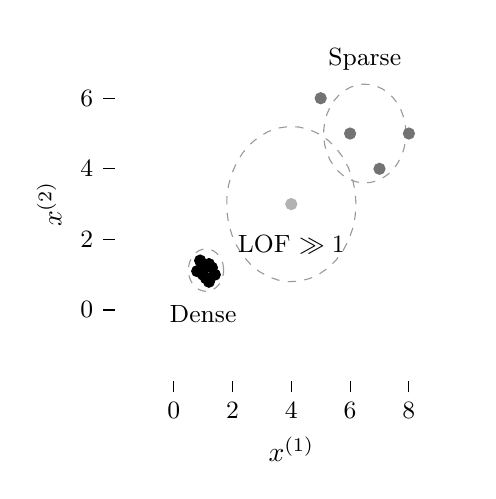
\begin{tikzpicture}
    \begin{axis}[
        xlabel={$x^{(1)}$}, ylabel={$x^{(2)}$},
        xmin=-2, xmax=10, ymin=-2, ymax=8,
        width=0.5\textwidth, height=0.5\textwidth,
        axis line style={draw=none},
        tick style={black, thin},
        xtick={0,2,4,6,8}, ytick={0,2,4,6},
        xticklabel style={font=\small},
        yticklabel style={font=\small},
        tick align=outside, tick pos=left,
    ]
    \addplot[only marks, mark=*, mark size=2pt, black] coordinates {
        (1,1) (1.2,1.3) (0.8,1.1) (1.1,0.9) (1.3,1.2)
        (0.9,1.4) (1.4,1.0) (1.0,1.2) (1.2,0.8)
    };
    \addplot[only marks, mark=*, mark size=2pt, black!55] coordinates {
        (6,5) (7,4) (5,6) (8,5)
    };
    \addplot[only marks, mark=*, mark size=2pt, black!30] coordinates {(4,3)};
    \addplot[black!40, dashed, thin, domain=0:360, samples=40]
        ({1.1 + 0.6*cos(x)}, {1.13 + 0.6*sin(x)});
    \addplot[black!40, dashed, thin, domain=0:360, samples=40]
        ({6.5 + 1.4*cos(x)}, {5.0 + 1.4*sin(x)});
    \addplot[black!40, dashed, thin, domain=0:360, samples=40]
        ({4 + 2.2*cos(x)}, {3 + 2.2*sin(x)});
    \node[font=\small, anchor=north] at (axis cs:1,0.4) {Dense};
    \node[font=\small, anchor=south] at (axis cs:6.5,6.5) {Sparse};
    \node[font=\small, anchor=north] at (axis cs:4,2.4) {LOF $\gg 1$};
    \end{axis}
\end{tikzpicture}
\caption{LOF detects the grey anomaly between two clusters of different density. Each dashed circle is a $k$-th-nearest-neighbour radius, scaled to the local density. The anomaly's circle is much larger than its neighbours' circles, so its LOF is far above $1$. A global $k$-NN distance threshold would either miss this point or flag the entire sparse cluster.}
\label{fig:lof_example}
\end{figure}

\vspace{2.5em}
\newthought{Reconstruction-based scoring.}\index{reconstruction error}\index{VAE!anomaly detection}
The third family reuses the bottleneck idea from chapter 6: train a model to reconstruct normal data, then score new inputs by how poorly they survive a round trip through the bottleneck.

\marginnote{\newthought{If the model cannot reconstruct it,} it has probably never seen anything like it. Reconstruction error is the most direct readout of representational familiarity.}

\newthought{Autoencoder reconstruction error}\index{autoencoder}\index{reconstruction error} provides a natural anomaly score.
Train an autoencoder on normal data only, then score each test point by how poorly it reconstructs:

\begin{align*}
    \mathrm{score}(x) &= \|x - \mathrm{decode}(\mathrm{encode}(x))\|^2
\end{align*}

High reconstruction error indicates the model has not learned to represent this type of input.
The score is interpretable in the same units as the input space, which makes thresholding straightforward.

\newthought{VAE log-likelihood}\index{VAE!anomaly detection}\index{ELBO}\index{KL divergence} refines the idea by using the negative ELBO from chapter 6 as the anomaly score:

\begin{align*}
    \mathrm{score}(x) &= -\mathrm{ELBO}(x) \\
                      &= -\mathbb{E}_{q(z \mid x)}[\log p(x \mid z)] + D_{\mathrm{KL}}\!\bigl(q(z \mid x) \,\|\, p(z)\bigr)
\end{align*}

An anomalous input both reconstructs poorly and requires an unusual latent encoding, contributing to both terms.
The KL term penalises latent codes far from the prior, so an input that the encoder maps to a region the prior almost never visits will rack up a large KL contribution even before reconstruction is considered.

\begin{figure}
\centering
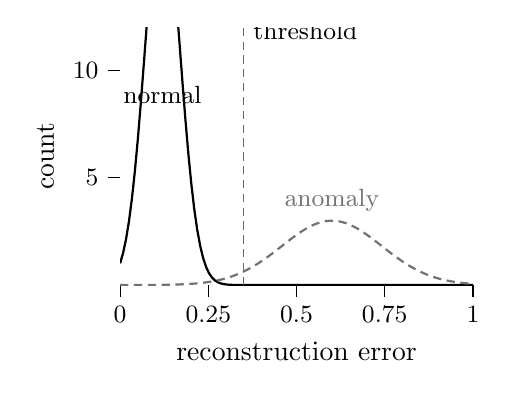
\begin{tikzpicture}
    \begin{axis}[
        xlabel={reconstruction error}, ylabel={count},
        xmin=0, xmax=1, ymin=0, ymax=12,
        width=0.5\textwidth, height=0.4\textwidth,
        axis line style={draw=none},
        tick style={black, thin},
        xtick={0,0.25,0.5,0.75,1}, ytick={5,10},
        xticklabel style={font=\small},
        yticklabel style={font=\small},
        tick align=outside, tick pos=left,
        samples=120, domain=0:1,
    ]
    \addplot[black, thick] {18*exp(-((x-0.12)^2)/0.005)};
    \addplot[black!55, thick, densely dashed] {3*exp(-((x-0.6)^2)/0.04)};
    \draw[densely dashed, black!60] (axis cs:0.35,0) -- (axis cs:0.35,12);
    \node[font=\small, anchor=south west] at (axis cs:0.35,11) {threshold};
    \node[font=\small, anchor=south] at (axis cs:0.12,8) {normal};
    \node[font=\small, black!55, anchor=south] at (axis cs:0.6,3) {anomaly};
    \end{axis}
\end{tikzpicture}
\caption{Reconstruction error distribution. Solid: errors on normal points cluster near zero. Dashed: errors on anomalies form a heavier-tailed distribution at higher values. The threshold separates the two; the operating point trades false positives for false negatives.}
\label{fig:reconstruction_histogram}
\end{figure}

\vspace{2.5em}
\newthought{Out-of-distribution scoring.}\index{OOD detection}\index{softmax confidence}
The fourth family handles the special case where the input may not even be drawn from the training distribution at all.

\marginnote{\newthought{OOD detection} formalises the question: is this input from the training distribution at all? Anomaly detection asks for outliers within a distribution; OOD asks whether the distribution itself applies.}

\newthought{Where anomaly detection asks whether a point deviates from the training distribution,} out-of-distribution detection frames this as a binary decision problem: in-distribution or out.
The distinction matters because OOD methods are designed for the regime where the input is so far from the training data that the model's learned representations may be entirely unreliable.

\newthought{Softmax confidence}\index{softmax confidence} is the naive baseline: flag inputs where $\max_k\, p(y{=}k \mid x)$ is low.
The problem is that neural networks are often confidently wrong on OOD data; the softmax normalises to sum to one regardless of how far the input is from any training example.
A flat softmax means the model is unsure between known classes; a peaked softmax says nothing about whether the input is a known class at all.

\newthought{ODIN}\index{ODIN}\index{temperature scaling}\cite{LiangODIN2018} improves on softmax confidence by combining temperature scaling with input perturbation:

\begin{align*}
    \tilde{x} &= x - \epsilon \cdot \mathrm{sign}\!\bigl(\nabla_x \log p(y{=}\hat{y} \mid x;\, T)\bigr)
\end{align*}

The temperature $T$ flattens the softmax during scoring, and the perturbation pushes the input slightly toward what the network expected; in-distribution inputs respond to the perturbation by rising in confidence, OOD inputs do not.

\newthought{Energy-based OOD detection}\index{energy score}\index{free energy}\cite{LiuEnergy2020} uses the free energy of the logits directly:

\begin{align*}
    E(x) &= -\log \sum_k \exp\!\bigl(f_k(x)\bigr)
\end{align*}

Higher energy indicates OOD.
Unlike softmax confidence, the energy score is not normalised to sum to one, so it can distinguish low-density regions of the logit space from high-density ones; an input with all logits close to zero produces a different energy than an input with one logit far above the others, even though their softmax probabilities may look similar.

\begin{figure}
\centering
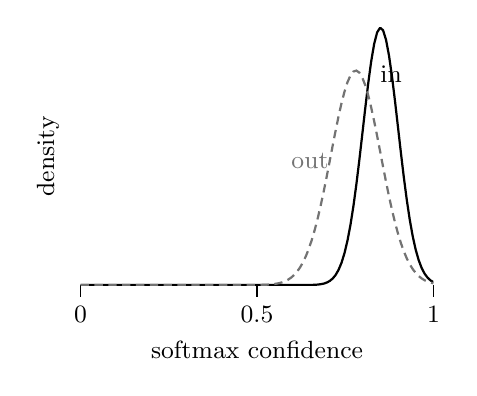
\begin{tikzpicture}
    \begin{axis}[
        xlabel={softmax confidence}, ylabel={density},
        xmin=0, xmax=1, ymin=0, ymax=12,
        width=0.5\textwidth, height=0.4\textwidth,
        axis line style={draw=none},
        tick style={black, thin},
        xtick={0,0.5,1}, ytick=\empty,
        xticklabel style={font=\small},
        xlabel style={font=\small},
        ylabel style={font=\small},
        tick align=outside, tick pos=left,
        samples=120, domain=0:1,
    ]
    \addplot[black, thick] {12*exp(-((x-0.85)^2)/0.005)};
    \addplot[black!55, thick, densely dashed] {10*exp(-((x-0.78)^2)/0.01)};
    \node[font=\small, anchor=south] at (axis cs:0.88,9) {in};
    \node[font=\small, black!55, anchor=south] at (axis cs:0.65,5) {out};
    \end{axis}
\end{tikzpicture}
\caption{Softmax confidence histogram on in-distribution inputs (solid) and OOD inputs (dashed). Both distributions peak at high confidence; the OOD peak is only slightly lower than the in-distribution peak, and the two overlap heavily. A threshold on softmax cannot cleanly separate the two families.}
\label{fig:ood_softmax}
\end{figure}

\begin{figure}
\centering
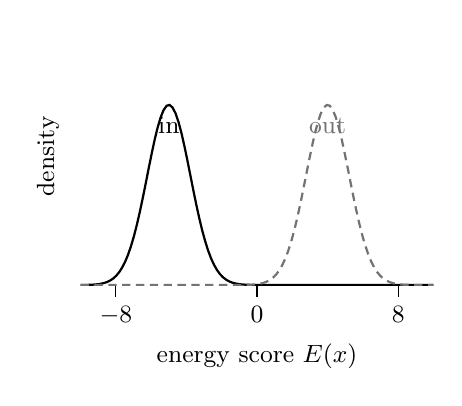
\begin{tikzpicture}
    \begin{axis}[
        xlabel={energy score $E(x)$}, ylabel={density},
        xmin=-10, xmax=10, ymin=0, ymax=10,
        width=0.5\textwidth, height=0.4\textwidth,
        axis line style={draw=none},
        tick style={black, thin},
        xtick={-8,0,8}, ytick=\empty,
        xticklabel style={font=\small},
        xlabel style={font=\small},
        ylabel style={font=\small},
        tick align=outside, tick pos=left,
        samples=120, domain=-10:10,
    ]
    \addplot[black, thick] {7*exp(-((x+5)^2)/3)};
    \addplot[black!55, thick, densely dashed] {7*exp(-((x-4)^2)/3)};
    \node[font=\small, anchor=south] at (axis cs:-5,5.5) {in};
    \node[font=\small, black!55, anchor=south] at (axis cs:4,5.5) {out};
    \end{axis}
\end{tikzpicture}
\caption{Energy score histogram for the same inputs. Because energy is not normalised, OOD inputs settle at distinctly higher (less negative) values, and the two distributions separate cleanly. The same network produces both Figure~\ref{fig:ood_softmax} and this figure; only the readout differs.}
\label{fig:ood_energy}
\end{figure}

\marginnote{\newthought{The softmax trap.} Softmax always sums to one. A network confidently wrong on a noise pattern produces a peaked softmax just as easily as one confidently right on a training image. Anything that bottoms out at the same maximum value cannot distinguish "I have seen this and it is class $k$" from "I have not seen this, but if I had to pick, I would pick class $k$".}


\subsection{Other Routes to OOD Detection}\index{misc class}\index{OOD detection}\index{reconstruction error}

\marginnote{\newthought{Three pragmatic routes} sit alongside the scoring methods above: bake the OOD problem into the label set, bolt on a dedicated detector head, or repurpose a generative model trained for something else.}

\newthought{The scoring methods so far} read uncertainty out of a classifier that was trained to do something else, and they all share a quiet assumption that the classifier's logits or its hidden representations carry usable signal about whether the input belongs at all.
Three alternative routes drop that assumption and ask the OOD question more directly, each with a different price tag.
They are worth knowing because in deployment the cheapest route is rarely the one that scores best on a benchmark, and the choice between them is usually decided by what data you can collect rather than by which estimator is most elegant.

\newthought{Add a misc class}\index{misc class}\cite{Hendrycks2017Baseline} is the simplest move available.
Train a $K{+}1$ class classifier where the extra class is a curated bucket of inputs the operator does not care about, things like blurred frames, sensor dropouts, or images from adjacent but irrelevant domains.
At inference the network simply predicts class $K{+}1$ for inputs that look like the bucket, and downstream code routes them to the same place an OOD score would.
The trade-off is unflattering once you spell it out: the misc class only catches what was put into it.
Anything operators did not anticipate, the network never sees a label for, so the OOD problem has not been solved, only reframed as an in-distribution problem with a new class whose recall is bounded by the imagination of whoever assembled the training set.

\newthought{A separate detector head}\index{detector head}\index{one-class learning} pushes the same idea one rung further by training an auxiliary binary head on top of the existing backbone\cite{Chandola2009}, with the explicit job of predicting in-distribution membership rather than class identity.
The head can be a one-class classifier fit on the training features, a small two-class network using a curated outlier set as negatives, or a logistic readout on a fixed penultimate layer.
This is essentially the learn-the-likelihood-of-being-correct idea pushed one step further, instead of predicting whether the prediction is correct, the head predicts whether the prediction even applies.
The route is cheap to add because the backbone is reused, but the detector inherits whatever blind spots the backbone has already baked in, and its quality is set almost entirely by where the boundary data come from.

\newthought{Reuse the VAE} from chapter 6 by treating the negative ELBO, or just the reconstruction term or the KL term to the prior, as a per-input OOD score\cite{KingmaWelling2014}.
A model that learned a tight latent representation of the training distribution should reconstruct training-like inputs cheaply and pay a visible reconstruction or KL cost on inputs from elsewhere.
This is the same machinery used as an anomaly score in the previous subsection, repurposed as an OOD test by changing what we count as a positive: not just outliers within the training distribution, but any input the generative model finds expensive to explain.
The route is fully unsupervised in the sense that no OOD labels are needed at training time, only the same reconstruction objective the VAE was trained with anyway.

\newthought{The familiar failure mode} of the reconstruction route is that visual neighbours of training classes still reconstruct cheaply, which we will pick up in the next subsection under the reconstruction-based blindness beat.
A held-out class that shares strokes, textures, or low-level features with training classes will travel through the bottleneck without much resistance, the score stays moderate, and the OOD test silently fails.
Reconstruction is sensitive to visual similarity, not to semantic membership, and the gap between the two is exactly where the route breaks.

\newthought{Comparing the three routes} clarifies when to reach for which.
The misc class is supervised and fragile: it works exactly as well as the curation behind it, and it pretends an open-set problem is closed.
The separate detector head is cheap and modular but inherits the backbone's biases, so a feature space that already collapses two domains together cannot be rescued by a head that reads off it.
The reconstruction score is fully unsupervised but answers a slightly different question, namely whether the input is hard to compress, which is only a proxy for whether it is hard to classify.
None of the three dominates in general, and a deployed system often runs two of them together so their failure modes are uncorrelated.

\marginnote{\newthought{A practical recipe.} Start with the misc class if you already have a curated bucket of nuisance inputs; add a separate detector head when the backbone is frozen and you cannot retrain end to end; fall back to the VAE reconstruction score when no labelled OOD data exist at all. Combining two routes covers more of the failure surface than tuning one of them harder.}


\subsection{When These Methods Fail}\index{calibration}\index{distribution shift}

\marginnote{\newthought{Every uncertainty method} inherits the model's notion of normal from the training data. When that notion is wrong or out of date, the detector silently degrades.}

\newthought{Every uncertainty method inherits the model's notion of normal from the training data.}
Failure modes follow predictably from where that inheritance breaks: the data shifts over time, the calibration drifts, the model is structurally blind to certain anomalies, the threshold is hard to set.

\newthought{Distribution shift}\index{distribution shift} is the most common and the hardest to detect.
A fraud detector trained on last year's transactions starts the new year well-calibrated, but consumer behaviour drifts, new payment products appear, fraud schemes evolve.
The detector keeps working as designed; it just no longer works for the world it now lives in.
The variance of MC Dropout still reflects what the model saw in training, not what the world looks like today, and the gap grows silently until losses force a relabel.

\begin{figure}
\centering
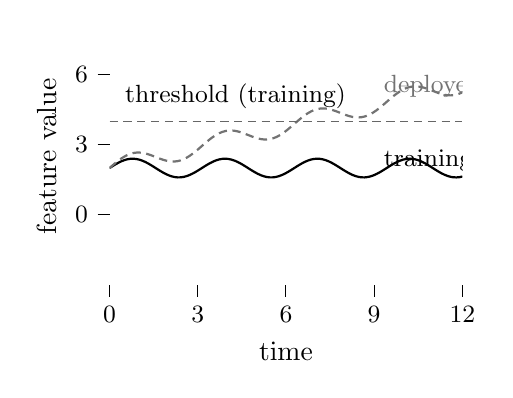
\begin{tikzpicture}
    \begin{axis}[
        xlabel={time}, ylabel={feature value},
        xmin=0, xmax=12, ymin=-3, ymax=8,
        width=0.5\textwidth, height=0.4\textwidth,
        axis line style={draw=none},
        tick style={black, thin},
        xtick={0,3,6,9,12}, ytick={0,3,6},
        xticklabel style={font=\small},
        yticklabel style={font=\small},
        tick align=outside, tick pos=left,
        samples=120, domain=0:12,
    ]
    \addplot[black, thick] {2 + 0.4*sin(deg(2*x))};
    \addplot[black!55, thick, densely dashed] {2 + 0.3*x + 0.4*sin(deg(2*x))};
    \draw[densely dashed, black!60] (axis cs:0,4) -- (axis cs:12,4);
    \node[font=\small, anchor=south west] at (axis cs:0.2,4.1) {threshold (training)};
    \node[font=\small, anchor=west] at (axis cs:9,2.3) {training};
    \node[font=\small, black!55, anchor=west] at (axis cs:9,5.5) {deployed};
    \end{axis}
\end{tikzpicture}
\caption{A feature drifts over time. The threshold set during training (dashed horizontal) becomes uninformative as the deployed-time distribution slides upward. The detector still uses the old threshold; the world no longer respects it.}
\label{fig:distribution_drift}
\end{figure}

\newthought{Calibration drift}\index{calibration!drift} compounds the shift problem.
Even when the underlying classes do not change, a model deployed long enough sees its predicted probabilities decouple from empirical frequencies as the input distribution drifts.
A $90\%$ confidence prediction may correspond to $90\%$ accuracy at deployment time and to $70\%$ accuracy six months later; without periodic recalibration on fresh labelled data, the uncertainty signal becomes a number that no longer means what it says.

\newthought{Reconstruction-based blindness}\index{failure modes!reconstruction} hits a different surface.
An autoencoder trained on MNIST digits zero through eight will reconstruct a held-out nine surprisingly well, because nines share local strokes with fours and sevens that the model has learned to encode.
The reconstruction error is moderate, the threshold sees nothing unusual, and the anomaly slips through.
The failure is not in the score; it is in the assumption that visual similarity equals familiarity.

\newthought{The threshold problem}\index{threshold!anomaly detection} is the practical headache that haunts every method.
In the absence of labelled anomalies, where exactly do we draw the line above which an input is flagged?
Set the threshold too tight and every input is flagged, drowning the operator in noise.
Set it too loose and real anomalies slip through.
The $k$-distance plot from chapter 4 had its own version of this; here we sweep the threshold across the score distribution and read off the operating point that balances false positives against true positives.

\begin{figure}
\centering
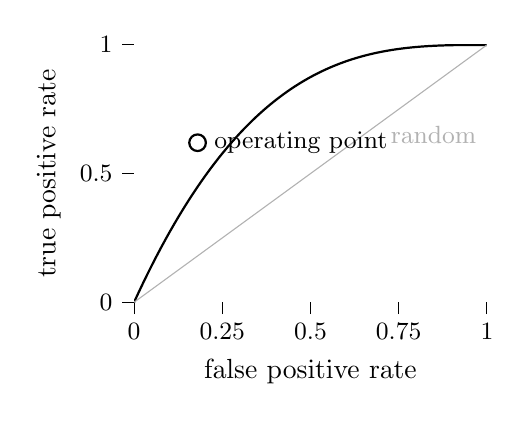
\begin{tikzpicture}
    \begin{axis}[
        xlabel={false positive rate}, ylabel={true positive rate},
        xmin=0, xmax=1, ymin=0, ymax=1,
        width=0.5\textwidth, height=0.4\textwidth,
        axis line style={draw=none},
        tick style={black, thin},
        xtick={0,0.25,0.5,0.75,1}, ytick={0,0.5,1},
        xticklabel style={font=\small},
        yticklabel style={font=\small},
        tick align=outside, tick pos=left,
        samples=80, domain=0:1,
    ]
    \addplot[black, thick] {1 - (1-x)^3};
    \addplot[black!30, thin] coordinates {(0,0) (1,1)};
    \addplot[only marks, mark=o, mark size=3pt, black, thick] coordinates {(0.18, 0.62)};
    \node[font=\small, anchor=west] at (axis cs:0.20,0.62) {operating point};
    \node[font=\small, black!30, anchor=west] at (axis cs:0.7,0.65) {random};
    \end{axis}
\end{tikzpicture}
\caption{Receiver operating characteristic\index{ROC curve} for an anomaly detector. The curve sweeps the threshold from strict (low FPR, low TPR) to loose (high FPR, high TPR). The open marker is one operating point chosen by domain cost: a false positive costs a human review; a false negative costs an undetected anomaly.}
\label{fig:roc_curve}
\end{figure}

\marginnote{\newthought{Stability analysis.}\index{stability analysis} Re-train the same detector on bootstrap subsamples of the training set and compare the flagged sets. Stable flags suggest genuine anomalies; flags that appear in only a few re-runs reflect detector variance, not signal. Stability is also a useful drift detector: a sudden drop in flag stability over time often precedes calibration failure.}

\newthought{When uncertainty estimates struggle,} the shared root cause is always the same: every method models normality from the training data, and the training data drifts.
The cure is operational: monitor the score distributions over time, recalibrate periodically, accept that no detector is permanent.
The next subsection turns these limits into a practical safety net.


\subsection{Acting Under Uncertainty: Graceful Degradation}\index{graceful degradation}\index{human handoff}

\marginnote{\newthought{Safe AI} means knowing when to hand off to a human. The four strategies in this subsection compose into a complete safety net.}

\newthought{Quantifying uncertainty is only useful if we act on it.}
Deployed ML systems must handle the inevitable cases they cannot confidently resolve; the difference between a fragile system and a robust one is whether the response to high uncertainty is documented in the architecture or improvised by the operations team.
Four strategies compose into a practical safety net.
They are not alternatives but layers; a well-engineered deployment uses all four together.

\newthought{Confidence thresholds}\index{confidence threshold} are the first layer.
The system acts autonomously only on predictions above a calibrated confidence level; everything else is escalated.
Picking the threshold is the practical work, and it is rarely a single number across all classes.
A medical triage classifier may demand $95\%$ confidence on positive predictions (acting on a positive ties up specialist time) and only $80\%$ on negative ones (a missed positive is far costlier than an over-cautious flag).
The threshold is a cost decision, not a statistical one.

\newthought{Human handoff}\index{human handoff} is the second layer.
Route uncertain or high-stakes cases to human reviewers.
Consider a radiology pipeline: an MRI image is fed to the model, MC Dropout returns a tumour probability with high epistemic variance because the lesion sits at the boundary between two morphologies the model has seen separately but never together.
The system does not return a yes/no decision; it queues the image for radiologist review with the model's prediction and uncertainty surfaced as context.
The radiologist confirms or overrides; the new label feeds back into the next training round, and the model's epistemic variance on similar images drops over time.

\newthought{Fail-safe defaults}\index{fail-safe defaults} are the third layer.
When uncertain, take the conservative action.
Consider an autonomous vehicle approaching an intersection where the lane-marking model returns high uncertainty: weather has worn the markings, the model has not seen this exact configuration.
The system does not guess at lane geometry; it falls back to a conservative behaviour like reducing speed and centering on the visible road edge until the uncertainty drops or a human driver intervenes.
The fail-safe is the action that costs least if the model is wrong.

\newthought{Monitoring}\index{monitoring} is the fourth layer, and the one most often skipped.
Track prediction confidence and anomaly scores over time, alerting when the score distribution shifts or the variance grows.
Drift in the input distribution shows up first as drift in the uncertainty distribution; a fraud detector whose mean confidence falls slowly over a quarter is telling you that the input distribution has moved, often weeks before the false-negative rate becomes visible.

\begin{figure}
\centering
\begin{tikzpicture}[
    every node/.style={font=\small, align=center},
    block/.style={rectangle, draw=black, thick, rounded corners=2pt,
                  minimum width=2.4cm, minimum height=0.7cm, inner sep=4pt},
    decide/.style={diamond, draw=black, thick, aspect=2,
                   minimum width=2.4cm, minimum height=0.7cm, inner sep=2pt},
    arr/.style={-{Triangle[length=4pt, width=4pt, fill=black!70]}, thick, black!70},
]
    \node[block] (input) at (0,4) {input $x$};
    \node[block, below=14pt of input, fill=black!8] (model) {model + uncertainty};
    \node[decide, below=16pt of model] (low) {low?};
    \node[decide, right=22pt of low] (med) {medium?};
    \node[block, below=22pt of low, minimum width=2cm] (act) {act};
    \node[block, right=10pt of act, minimum width=2.2cm] (fallback) {fail-safe};
    \node[block, right=10pt of fallback, minimum width=2.2cm] (handoff) {human};
    \node[block, below=20pt of fallback, minimum width=6.4cm] (monitor) {monitor over time};

    \draw[arr] (input) -- (model);
    \draw[arr] (model) -- (low);
    \draw[arr] (low) -- node[left, font=\tiny] {yes} (act);
    \draw[arr] (low) -- node[above, font=\tiny] {no} (med);
    \draw[arr] (med) |- node[right, font=\tiny, pos=0.25] {yes} (fallback);
    \draw[arr] (med.east) -| node[above, font=\tiny, pos=0.25] {no} (handoff);
    \draw[arr] (act) |- (monitor);
    \draw[arr] (handoff) |- (monitor);
\end{tikzpicture}
\caption{Decision flow for a deployed model with uncertainty estimation. Low uncertainty: act autonomously. Medium uncertainty: fall back to a conservative default. High uncertainty: hand off to a human. All three branches feed into a monitoring layer that watches the score distribution over time and alerts on drift.}
\label{fig:degradation_flow}
\end{figure}

\marginnote{\newthought{Practical protocol.} Choose the confidence threshold from a held-out validation set with labelled errors, prioritising the cost asymmetry of your domain. Pick the fail-safe action so that, if invoked unnecessarily, it costs the least. Route to human review only when neither acting nor falling back is clearly correct. Monitor the rates of all three branches; sudden changes in routing share are a leading indicator of drift.}

\newthought{The payoff} of all this machinery is a system that can refuse to answer.
A model that answers everything is impressive in a demo and dangerous in production; a model that refuses on the cases it should refuse on is the one you can deploy and sleep through the night.
Uncertainty estimation, anomaly scoring, OOD detection, and graceful degradation are the four pieces that turn a confident classifier into a trustworthy one.


% ==============================================================================================
% BLOCK 3: STUDENT ACTIVATION
% ==============================================================================================

\newpage

\section{Examples \& Exercises}\index{examples}\index{exercises}

\marginnote{\newthought{Exercises} are for practice and reinforcing concepts. Try to solve them on your own first,
try things, play with it, discuss, this is not a time trial. And there is no shame in not ending up at the right answer,
in the same sense, that uncovering great questions
and tossing them around is usually pretty fruitful on the long run.}

\newthought{Computing by hand} builds the intuition that no anomaly score can replace.
Step through the arithmetic slowly.

\vspace{1em}

\newthought{Aleatoric versus epistemic identification.}
For each scenario below, classify the dominant source of uncertainty as aleatoric or epistemic, and propose the appropriate response in one sentence.

\begin{itemize}
    \item A handwriting recognition system encounters a digit that genuinely sits between a $4$ and a $9$ even to a human reader.
    \item A medical image classifier trained on adult patients receives its first paediatric scan.
    \item A speech recogniser deployed in a noisy factory mishears commands during machinery operation.
    \item A fraud detector trained on credit card data encounters its first cryptocurrency transaction.
    \item A weather model trained on temperate climates is asked to forecast a tropical cyclone.
\end{itemize}

\marginnote{\newthought{Sketch.} (1) Aleatoric: ambiguity is in the data, the optimal output is a probability over both classes. (2) Epistemic: the model has seen no paediatric data, more training data would close the gap. (3) Aleatoric: the noise floor of the input is the bottleneck. (4) Epistemic: a new product class never seen during training. (5) Epistemic: structural absence of relevant training data. The right response in (1) and (3) is to communicate the irreducible spread; in (2), (4), (5) it is to flag for review and collect labels.}

\vspace{2.5em}

\newthought{MC Dropout uncertainty.}
A classifier with dropout produces the following softmax outputs for a single input across $T{=}5$ forward passes:

\begin{table*}[ht]
\centering
\begin{tabular}{p{0.08\textwidth}p{0.10\textwidth}p{0.10\textwidth}}
    \toprule
    \textbf{Pass} & \textbf{$p(\text{cat})$} & \textbf{$p(\text{dog})$} \\
    \midrule
    1 & 0.9 & 0.1 \\
    2 & 0.4 & 0.6 \\
    3 & 0.7 & 0.3 \\
    4 & 0.5 & 0.5 \\
    5 & 0.8 & 0.2 \\
    \bottomrule
\end{tabular}
\vspace{2em}
\caption{Five MC Dropout forward passes for a single input. The mean leans toward cat, but the spread across passes is the signal that quantifies epistemic uncertainty.}
\label{tab:mc_dropout_passes}
\end{table*}

Compute the predictive mean and variance for $p(\text{cat})$.
Would you trust this prediction?
At what variance threshold would you route this input to a human reviewer?

\marginnote{%
\begin{align*}
    \bar{p} &= \tfrac{0.9 + 0.4 + 0.7 + 0.5 + 0.8}{5} \\
            &= \tfrac{3.3}{5} \\
            &= 0.66 \\[4pt]
    \mathrm{Var}(\hat{p}) &= \tfrac{1}{5}\sum_t (p_t - 0.66)^2 \\
                          &\approx \tfrac{0.0576+0.0676+0.0016+0.0256+0.0196}{5} \\
                          &\approx 0.034
\end{align*}%
The mean leans toward cat, but the variance is substantial; pass 2 disagrees strongly with the others. This input sits in a region of high epistemic uncertainty. A reasonable handoff threshold for binary classification is $\mathrm{Var}(\hat{p}) > 0.02$, which this input clearly crosses; route to a human reviewer.
}

\vspace{2.5em}

\newthought{Z-score by hand.}
A sensor returns readings with population mean $\mu{=}10$ and standard deviation $\sigma{=}2$.
For each test value, compute the z-score and decide whether it is anomalous under the rule $|z| > 3$.

\begin{itemize}
    \item $x_1 = 12$
    \item $x_2 = 17$
    \item $x_3 = 4$
\end{itemize}

The arithmetic for $x_1$:

\begin{align*}
    z_1 &= \frac{12 - 10}{2} \\
        &= \frac{2}{2} \\
        &= 1
\end{align*}

So $|z_1| = 1$ which is below the threshold; $x_1$ is not flagged.

Compute $z_2$ and $z_3$ yourself, then verify against the table below.

\begin{table*}[ht]
\centering
\begin{tabular}{p{0.10\textwidth}p{0.10\textwidth}p{0.10\textwidth}p{0.20\textwidth}}
    \toprule
    \textbf{Value} & \textbf{$z$} & \textbf{$|z| > 3$} & \textbf{Decision} \\
    \midrule
    $x_1 = 12$ & $1$  & no  & not anomalous \\
    $x_2 = 17$ & $3.5$ & yes & flag \\
    $x_3 = 4$  & $-3$ & at threshold & borderline \\
    \bottomrule
\end{tabular}
\vspace{2em}
\caption{Z-score classification for three test values under $\mu{=}10$, $\sigma{=}2$, threshold $|z|{>}3$.}
\label{tab:zscore_values}
\end{table*}

\marginnote{\newthought{Why the threshold breaks on heavy-tailed data.} A Gaussian assigns a probability of about $0.003$ to $|z| > 3$, so the rule is nominally a $0.3\%$ false-positive rate. On heavy-tailed data, the true probability of $|z| > 3$ can be ten times larger, so the same rule flags ten times more points than it should. The fix is to estimate the tail with EVT or to fit a heavier-tailed distribution.}

\vspace{2.5em}

\newthought{Gaussian Mixture Model likelihood.}
A two-component GMM is fit to a sensor stream with parameters $\pi_1{=}0.6$, $\mu_1{=}0$, $\sigma_1{=}1$, and $\pi_2{=}0.4$, $\mu_2{=}5$, $\sigma_2{=}1$.
Compute the likelihood of two test points: $x_a = 0.5$ (near component 1) and $x_b = 2.5$ (between components).

For $x_a$, the per-component contributions are:

\begin{align*}
    \pi_1 \, \mathcal{N}(0.5 \mid 0, 1) &= 0.6 \cdot \tfrac{1}{\sqrt{2\pi}} \exp\!\bigl(-\tfrac{0.25}{2}\bigr) \\
                                          &\approx 0.6 \cdot 0.352 \\
                                          &\approx 0.211 \\[4pt]
    \pi_2 \, \mathcal{N}(0.5 \mid 5, 1) &= 0.4 \cdot \tfrac{1}{\sqrt{2\pi}} \exp\!\bigl(-\tfrac{20.25}{2}\bigr) \\
                                          &\approx 0.4 \cdot 1.6\times10^{-5} \\
                                          &\approx 6.4\times10^{-6}
\end{align*}

So $p(x_a) \approx 0.211$.
Compute $p(x_b)$ yourself, then verify against the table.

\begin{table*}[ht]
\centering
\begin{tabular}{p{0.10\textwidth}p{0.18\textwidth}p{0.18\textwidth}p{0.14\textwidth}}
    \toprule
    \textbf{Point} & \textbf{$\pi_1\mathcal{N}_1$} & \textbf{$\pi_2\mathcal{N}_2$} & \textbf{$p(x)$} \\
    \midrule
    $x_a = 0.5$ & $0.211$  & $6.4\times10^{-6}$ & $0.211$ \\
    $x_b = 2.5$ & $0.0021$ & $0.0021$           & $0.0042$ \\
    \bottomrule
\end{tabular}
\vspace{2em}
\caption{GMM likelihoods. $x_a$ sits inside component 1 and earns a likelihood two orders of magnitude higher than $x_b$, which sits in the gap between the two components and earns approximately equal but small contributions from each.}
\label{tab:gmm_likelihood}
\end{table*}

\marginnote{\newthought{Reading the table.} The gap between two well-separated components is a low-likelihood region; an input there is anomalous in the sense that neither component explains it well. This is precisely the failure mode of fitting too few components: real variation gets flagged as anomaly. The fix is to validate $K$ on held-out data, not to set it once and forget.}

\vspace{2.5em}

\newthought{LOF by hand.}
Five points $x_1{=}(0,0)$, $x_2{=}(1,0)$, $x_3{=}(0,1)$, $x_4{=}(1,1)$, $x_5{=}(5,5)$ with $k{=}2$.
Compute the $2$-distance for each point (the distance to its second nearest neighbour) and decide which has the highest LOF.

The pairwise distances:

\begin{align*}
    d(x_1, x_2) &= \sqrt{1^2 + 0^2} = 1 \\
    d(x_1, x_3) &= \sqrt{0^2 + 1^2} = 1 \\
    d(x_1, x_4) &= \sqrt{1^2 + 1^2} = \sqrt{2} \approx 1.41 \\
    d(x_1, x_5) &= \sqrt{5^2 + 5^2} = \sqrt{50} \approx 7.07
\end{align*}

So $x_1$'s nearest neighbour is $x_2$ or $x_3$ (both at distance 1), and its $2$-distance (the second nearest) is also 1.

Compute the $2$-distance for the other points and verify against the table.

\begin{table*}[ht]
\centering
\begin{tabular}{p{0.08\textwidth}p{0.12\textwidth}p{0.16\textwidth}p{0.14\textwidth}p{0.14\textwidth}}
    \toprule
    \textbf{Point} & \textbf{Coords} & \textbf{Nearest 2 distances} & \textbf{$2$-distance} & \textbf{LOF} \\
    \midrule
    $x_1$ & $(0,0)$ & $1.00, 1.00$ & $1.00$ & $\approx 1$ \\
    $x_2$ & $(1,0)$ & $1.00, 1.00$ & $1.00$ & $\approx 1$ \\
    $x_3$ & $(0,1)$ & $1.00, 1.00$ & $1.00$ & $\approx 1$ \\
    $x_4$ & $(1,1)$ & $1.00, 1.00$ & $1.00$ & $\approx 1$ \\
    $x_5$ & $(5,5)$ & $5.66, 6.40$ & $6.40$ & $\gg 1$ \\
    \bottomrule
\end{tabular}
\vspace{2em}
\caption{LOF computation for five points with $k{=}2$. The four cluster points have $2$-distance $1.0$, identical local reachability density, and LOF near $1$. Point $x_5$ has $2$-distance $6.4$, much sparser local density, and LOF much greater than $1$, flagging it as an anomaly.}
\label{tab:lof_trace}
\end{table*}

\marginnote{\newthought{Why LOF beats global $k$-NN distance.} If we only used $x_5$'s distance to its nearest neighbour (about $5.66$), we would get a bare distance number, but no sense of how far that is relative to the local density elsewhere. LOF normalises by the density of the neighbours, so $x_5$'s sparseness is measured against the cluster's tightness. A point that is far in absolute terms but in a sparse region everywhere would have LOF near $1$ and not be flagged.}

\vspace{2.5em}

\newthought{Reconstruction anomaly.}
You train an autoencoder on MNIST digits zero through eight.
At test time, you present digit nine.
What reconstruction error do you expect?
Under what circumstances might the autoencoder still produce a low error, and what does that tell you about the limits of reconstruction-based detection?

\marginnote{\newthought{The visual-similarity trap.} The model never learned to encode or decode nines, so the reconstruction should be poor. However, nines share local features with fours (the diagonal) and sevens (the top stroke), so the autoencoder may reconstruct a nine as a visually plausible four or seven and earn only moderate error. The threshold sees nothing unusual, the anomaly slips through. Reconstruction-based detection works only when anomalies are visually different from any familiar class; structural near-neighbours of training classes are the standard failure mode.}

\vspace{2.5em}

\newthought{Energy versus softmax for OOD.}
A network trained on three classes returns logit vectors for two test inputs:

\begin{align*}
    f(x_{\mathrm{in}})  &= (3.0,\, 1.0,\, 0.5) \\
    f(x_{\mathrm{out}}) &= (1.2,\, 1.0,\, 0.9)
\end{align*}

Compute the softmax confidence (the maximum softmax probability) and the energy score $E(x) = -\log\sum_k \exp(f_k(x))$ for each input.

For $x_{\mathrm{in}}$, the softmax denominator is:

\begin{align*}
    \sum_k \exp(f_k) &= e^{3.0} + e^{1.0} + e^{0.5} \\
                     &\approx 20.09 + 2.72 + 1.65 \\
                     &\approx 24.46
\end{align*}

So $\max_k p(y{=}k \mid x_{\mathrm{in}}) = e^{3.0}/24.46 \approx 0.82$.
The energy is $E(x_{\mathrm{in}}) = -\log(24.46) \approx -3.20$.

Compute the same for $x_{\mathrm{out}}$ and verify:

\begin{table*}[ht]
\centering
\begin{tabular}{p{0.18\textwidth}p{0.16\textwidth}p{0.16\textwidth}p{0.18\textwidth}}
    \toprule
    \textbf{Input} & \textbf{$\sum_k \exp(f_k)$} & \textbf{Softmax max} & \textbf{Energy $E(x)$} \\
    \midrule
    $x_{\mathrm{in}}$  & $24.46$ & $0.82$ & $-3.20$ \\
    $x_{\mathrm{out}}$ & $9.28$  & $0.36$ & $-2.23$ \\
    \bottomrule
\end{tabular}
\vspace{2em}
\caption{Softmax confidence and energy for an in-distribution input and an OOD input. The softmax confidence drops from $0.82$ to $0.36$, but it stays well above zero. The energy is more diagnostic because it is not normalised: the OOD input has higher energy ($-2.23 > -3.20$), reflecting that the logit values are uniformly small.}
\label{tab:energy_softmax}
\end{table*}

\marginnote{\newthought{What the energy sees.} The softmax of $x_{\mathrm{out}}$ is flat, so the maximum is small, and a softmax-only detector would catch this case. But softmax stays peaked on adversarial inputs that push one logit very high; energy stays high because the absolute logit values, not just the relative ones, matter. The energy reads "I am confident" only when the logits have absolute magnitude.}

\vspace{2.5em}

\newthought{Threshold selection by ROC.}
An anomaly detector reports the following operating points across five candidate thresholds:

\begin{table*}[ht]
\centering
\begin{tabular}{p{0.10\textwidth}p{0.14\textwidth}p{0.14\textwidth}}
    \toprule
    \textbf{Threshold} & \textbf{FPR} & \textbf{TPR} \\
    \midrule
    $\tau_1$ (strict) & $0.02$ & $0.30$ \\
    $\tau_2$           & $0.08$ & $0.55$ \\
    $\tau_3$           & $0.18$ & $0.75$ \\
    $\tau_4$           & $0.35$ & $0.88$ \\
    $\tau_5$ (loose)   & $0.60$ & $0.95$ \\
    \bottomrule
\end{tabular}
\vspace{2em}
\caption{Five operating points for an anomaly detector, swept from strict (low FPR, low TPR) to loose. Each row is a different choice of threshold.}
\label{tab:roc_sweep}
\end{table*}

Sketch the ROC curve from these five points.
Suppose a false positive costs one unit of human review and a false negative costs ten units of undetected anomaly.
Which operating point minimises the expected total cost if anomalies make up $5\%$ of the inputs?

\marginnote{\newthought{Cost-aware operating point.} Let $p$ be the prior on anomalies. Expected cost per input is $\mathrm{cost} = (1-p)\cdot \mathrm{FPR}\cdot c_{\mathrm{FP}} + p\cdot(1-\mathrm{TPR})\cdot c_{\mathrm{FN}}$. With $p{=}0.05$, $c_{\mathrm{FP}}{=}1$, $c_{\mathrm{FN}}{=}10$: $\tau_1{:}\,0.95{\cdot}0.02{\cdot}1 + 0.05{\cdot}0.70{\cdot}10 = 0.36$; $\tau_2{:}\,0.30$; $\tau_3{:}\,0.30$; $\tau_4{:}\,0.39$; $\tau_5{:}\,0.62$. The minimum is at $\tau_2$ or $\tau_3$, around $0.30$ per input. Either is acceptable; $\tau_3$ catches more anomalies at slightly higher review cost, which is often the safer choice when $c_{\mathrm{FN}}$ is uncertain.}

\vspace{2.5em}

% ============================= CODE ===============================

\marginnote{\newthought{Code} will be provided as a Python notebook.
Use it as a starting point, break things, and observe what changes.}
\marginnote{500 sensor readings\\480 normal, 20 injected anomalies\\3-dimensional features\\[4pt]implement: $k$-NN distance, LOF, autoencoder reconstruction error, ROC sweep}

\newthought{A sensor dataset to explore.}
You are given 500 sensor readings from a manufacturing line, 480 normal and 20 injected anomalies of three different kinds: point anomalies far from the cluster, density-shift anomalies between two natural sub-clusters, and structural anomalies whose values are normal but whose feature combinations are unusual.
Apply $k$-NN distance, LOF, and autoencoder reconstruction error.
Compare the three anomaly-score distributions for normal versus anomalous points.
Sweep the threshold and plot the trade-off between false positives and detection rate for each method.

\newthought{What to observe.}
$k$-NN distance works well when the anomalies are globally far from normal data but struggles when a dense and a sparse cluster coexist; the global threshold has nowhere to sit.
LOF handles the density variation by normalising against local density and catches the density-shift anomalies the $k$-NN distance misses.
The autoencoder catches structural anomalies that are close in distance but structurally different from anything the model learned to encode, but it misses the visually similar ones for exactly the reason discussed in the LOF and reconstruction exercises.
No single method dominates across all anomaly types; the practical recipe is to ensemble them and route on agreement, falling back to human review when methods disagree.

\fi
\newthought{Self-Reflection} questions to guide your thinking:
\begin{itemize}
    \item Why does softmax turn confidence into a similarity score within the training distribution rather than an absolute correctness estimate?
    \item Why is high softmax confidence on an adversarial perturbation the same failure mode as overconfidence out of domain, not a separate one?
    \item In a reliability diagram, why does the gap at the heaviest bin determine the user-visible failure mode of a deployed system?
    \item Why does histogram binning close the in-domain ECE almost completely while leaving the out-of-domain ECE almost untouched?
    \item How does histogram binning differ in assumption and applicability from a separately trained confidence head?
    \item How does MC Dropout turn a single trained network into an estimator of predictive variance, and what assumption links that variance to epistemic uncertainty?
    \item Which kind of out-of-domain input is structurally invisible to MC Dropout, and why?
    \item In a DeVries-Taylor confidence head, every hint towards the label costs $-\log c$. Why does that loss alone tend to saturate at $c\!\to\!1$, and what does outlier exposure add that closes the loophole?
    \item Why can the reconstruction error of a one-class VAE flag an out-of-domain input even when its latent embedding falls inside the training cloud, and what kind of input slips through that signal?
    \item Why do VAE reconstruction error and VAE latent geometry tend to confuse the same out-of-domain inputs, and what does that say about geometric vs semantic OOD detection?
    \item What separates aleatoric from epistemic uncertainty, and which of the two is reduced by collecting more training data?
    \item Why does the heavy tail of real-world data imply that the epistemic component cannot be driven to zero, and what does that mean for safety-critical deployment?
    \item How do data drift and model drift, defined relative to the operational design domain, decouple stated confidence from empirical accuracy at runtime?
    \item Why can a one-class generator serve as an anomaly detector without ever observing a labelled anomaly, and what does that imply for the choice of objective?
    \item On what axes would you compare softmax, calibration, MC Dropout, a confidence head, and a VAE OOD score when picking one for a concrete deployment?
\end{itemize}

\newthought{Recap} of Key Concepts:
\begin{itemize}
    \item Softmax encodes similarity within the training distribution, not correctness, and so fails out of domain and on adversarial inputs.
    \item ECE measures the gap between stated confidence and empirical accuracy; histogram binning closes it on the distribution it was fit on but does not transfer.
    \item Uncertainty splits into aleatoric (irreducible noise) and epistemic (model ignorance); MC Dropout and a confidence head estimate the latter, and only the latter shrinks under more training data.
    \item A one-class VAE turns reconstruction error and latent geometry into OOD signals, and inherits a blind spot whenever the unknown looks geometrically like the known.
    \item The operational design domain delimits the input slice the model was trained for; data drift and model drift decouple stated confidence from empirical accuracy at runtime.
\end{itemize}


\newthought{A notion of domain.} Every method in this chapter inherits its notion of domain
from a narrow training distribution, and the long tail of novel inputs is structurally
invisible to a narrowly-trained detector. The data covers only an increment of the input
space the deployed model will encounter.

\newthought{Transfer learning.} In order to build ever more capable models and expand
beyond known domains, our target is to widen the feature space before a new domain or a
new task even arrives.

\marginnote{\newthought{Teaser.} How do our embeddings need to be formalized and trained in order to generalize and transfer between tasks and domains?}

\marginnote{\newthought{feedback}}
